\appendix

\section{Supporting tables and figures}

\begin{figure}[t]
\centering
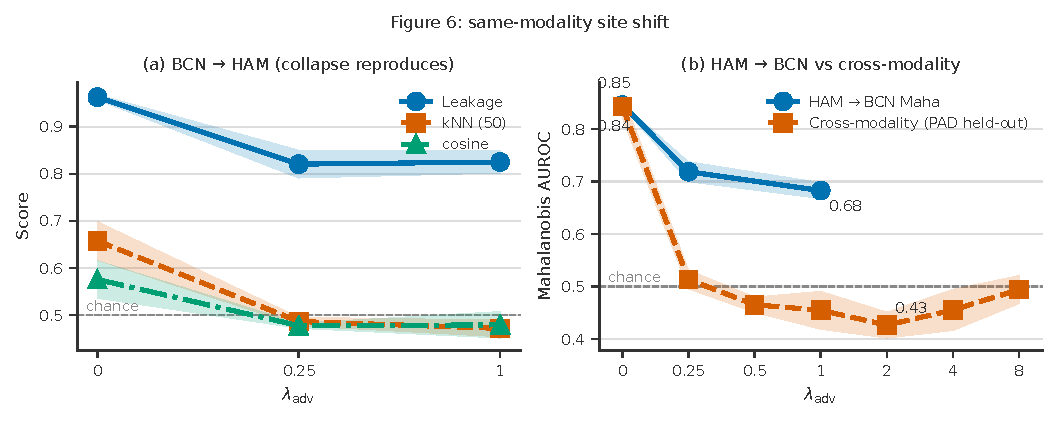
\includegraphics[width=\textwidth]{../../results/paperB/figures/fig6_site_shift.pdf}
\caption{\textbf{A same-modality site shift separates the two claims.} (a) Barcelona to
HAM10000: leakage falls and the detectors with headroom cross chance. (b) With the roles
reversed to restore headroom, Mahalanobis falls from a baseline matching the
cross-modality sweep but stops above chance, while the cross-modality sweep
continues below it.}
\label{fig:site}
\end{figure}

\begin{figure}[t]
\centering
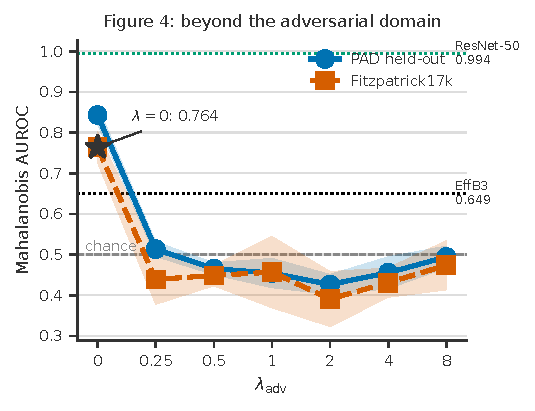
\includegraphics[width=\textwidth]{../../results/paperB/figures/fig4_generalises.pdf}
\caption{\textbf{The collapse is not confined to the adversarial domain.} AUROC against $\lam$
for the held-out PAD partition and for Fitzpatrick17k, which is absent from every
training branch. Horizontal references give the ResNet-50 baseline and the
EfficientNet-B3 control on Fitzpatrick; the controlled comparison is the $\lam = 0$
point of the sweep itself.}
\label{fig:gen}
\end{figure}

\begin{figure}[t]
\centering
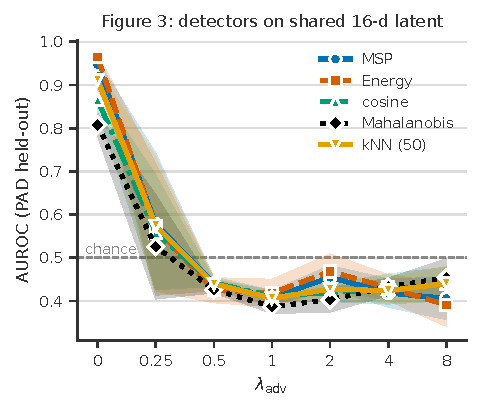
\includegraphics[width=0.72\textwidth]{../../results/paperB/figures/fig3_detectors.pdf}
\caption{\textbf{Every scoring rule moves together.} The five detectors against $\lam$ on the
held-out PAD partition, mean $\pm$ 1 s.d. All five are functions of the same
16-dimensional latent and are therefore not independent evidence;
Figure~\ref{fig:depth} carries the replication on a different representation.}
\label{fig:det}
\end{figure}

\begin{figure}[t]
\centering
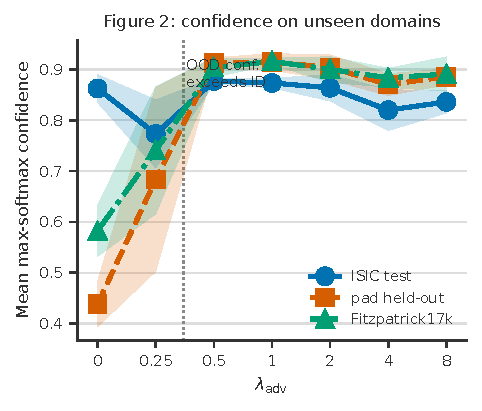
\includegraphics[width=\textwidth]{../../results/paperB/figures/fig2_confidence.pdf}
\caption{\textbf{Confidence on unseen domains overtakes confidence on familiar data.} Mean
maximum-softmax probability against $\lam$ for the ISIC test split, the held-out PAD
partition and Fitzpatrick17k. The crossing occurs by $\lam \approx 0.5$. $\lambda$
spacing is categorical.}
\label{fig:conf}
\end{figure}

\begin{figure}[t]
\centering
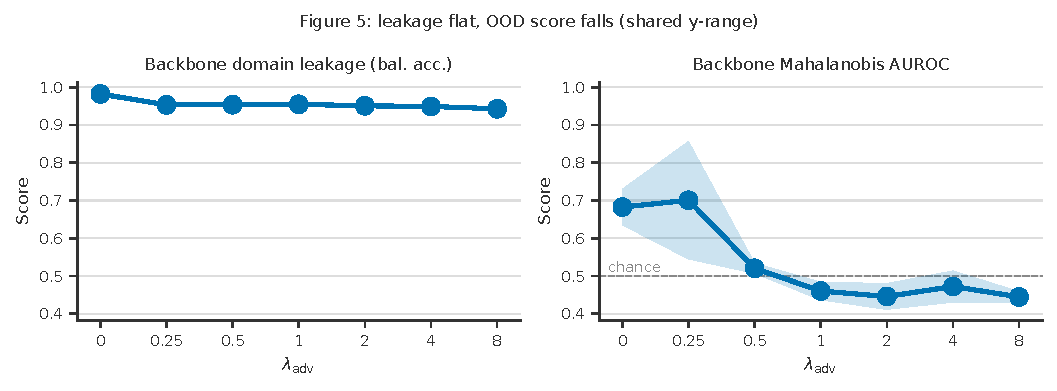
\includegraphics[width=\textwidth]{../../results/paperB/figures/fig5_leakage_no_mediation.pdf}
\caption{\textbf{Leakage does not mediate the collapse.} At the pre-projection backbone the
domain probe stays flat across the sweep while Mahalanobis AUROC falls. Domain
information remains linearly decodable and detection degrades regardless.}
\label{fig:depth}
\end{figure}

\begin{table}[t]
\centering
\small
\caption{Invariance objectives other than gradient reversal, single-encoder backbone,
3 seeds per cell. Leakage is balanced accuracy, floor $0.5$. \textbf{IRM and GroupDRO
use PAD labels} through their environment and group risks; the remaining objectives do
not, so their cross-domain numbers are not comparable and the two regimes are kept in
separate blocks.}
\label{tab:obj}
\begin{tabular}{llcccc}
\toprule
Objective & Weight & Leakage & Maha.\ AUROC & ID bal.\ acc & OOD ECE \\
\midrule
\multicolumn{6}{l}{\emph{No access to PAD labels}}\\
ERM\rlap{$^{\S}$} & ---    & 0.973 & 0.838 & 0.761 & --- \\
CORAL        & 100    & 0.998 & 0.999 & 0.777 & --- \\
MMD          & 1      & 0.967 & 0.813 & 0.779 & --- \\
MMD          & 100    & 0.900 & 0.716 & 0.730 & --- \\
MMD          & 3000   & 0.893 & 0.748 & 0.382 & 0.142 \\
MMD          & 10000  & 0.836 & 0.665 & 0.337 & 0.267 \\
\textbf{GRL} & $\lam = 0.25$ & \textbf{0.763} & \textbf{0.525} & \textbf{0.845\rlap{$^\dagger$}} & --- \\
\midrule
\multicolumn{6}{l}{\emph{Uses PAD labels --- not comparable on cross-domain accuracy}}\\
IRM          & 100    & 0.950 & 0.729 & 0.167 & --- \\
GroupDRO     & 10     & 0.976 & 0.868 & 0.783 & --- \\
\bottomrule
\multicolumn{6}{l}{\footnotesize $^\dagger$ plain accuracy for the GRL row; see Table~\ref{tab:single}.}\\
\multicolumn{6}{l}{\footnotesize $^{\S}$ scored on \texttt{pad\_full} with a uniform optimiser and an ISIC-only loss; the}\\
\multicolumn{6}{l}{\footnotesize \phantom{$^{\S}$} $\lam{=}0$ row of Table~\ref{tab:single} uses \texttt{pad\_heldout}, grouped learning rates and}\\
\multicolumn{6}{l}{\footnotesize \phantom{$^{\S}$} \texttt{ignore\_index}. They are not the same condition. \pending{harmonise or relabel.}}
\end{tabular}
\end{table}

\begin{table}[t]
\centering
\small
\caption{Single-encoder DANN on the same data and splits. ID accuracy is plain accuracy;
leakage is balanced accuracy, floor $0.5$. All five detectors collapse at the smallest
non-zero weight, and four of five fall below chance by $\lam = 4$.}
\label{tab:single}
\begin{tabular}{lccccccccc}
\toprule
$\lam$ & $n$ & Leakage & Maha. & $k$-NN & MSP & cosine & Energy & ID acc & X-dom \\
\midrule
0    & 5 & 0.970 & 0.700 & \textbf{0.944} & 0.868 & 0.884 & \textbf{0.911} & 0.845 & 0.390 \\
0.25 & 3 & \textbf{0.763} & 0.525 & \textbf{0.528} & 0.515 & 0.509 & \textbf{0.507} & 0.845 & 0.333 \\
0.5  & 3 & 0.795 & 0.510 & 0.517 & 0.501 & 0.493 & 0.507 & 0.844 & 0.328 \\
1    & 3 & 0.795 & 0.548 & 0.521 & 0.462 & 0.482 & 0.448 & 0.840 & 0.334 \\
2    & 5 & 0.807 & 0.509 & 0.516 & 0.479 & 0.468 & 0.470 & 0.839 & 0.325 \\
4    & 3 & 0.798 & 0.502 & 0.486 & 0.471 & 0.454 & 0.449 & 0.835 & 0.320 \\
8    & 3 & 0.787 & 0.520 & 0.532 & 0.519 & 0.490 & 0.500 & 0.832 & 0.321 \\
\bottomrule
\end{tabular}
\end{table}

\begin{table}[t]
\centering
\small
\caption{Candidate explanations tested and refuted. Each was a prediction specified
before its test.}
\label{tab:refuted}
\begin{tabular}{p{3.1cm}p{5.2cm}p{6.1cm}}
\toprule
Explanation & Test & Result \\
\midrule
Memorisation of the adversarial images & Hold PAD out of the adversary at patient level & \texttt{pad\_heldout} $0.427$ vs \texttt{pad\_adv} $0.407$; unchanged \\
Class composition & Restrict ID to the six shared classes; reweight ID to the OOD class mix & $0.432$ vs $0.427$ on \texttt{pad\_heldout}; reweighting \emph{strengthens} the inversion to $0.259$ \\
Domain specificity & Evaluate on Fitzpatrick17k, never in $\mathcal{L}_{\mathrm{adv}}$ & $0.391$ at $\lam = 2$ against $0.764$ at $\lam = 0$, same model and data \\
Dimensional collapse & Participation ratio and eigenspectrum across $\lam$ & $4.879 \to 4.500$ while leakage $0.914 \to 0.553$ (same three runs); decoupled \\
Latent compression & Latent variance and distance to centroid across $\lam$ & OOD is already $4.5\times$ tighter at $\lam = 0$; the adversary \emph{decompresses} it \\
Tail asymmetry & Recompute AUROC after truncating the pooled upper tail & $0.412$--$0.424$ versus $0.427$; medians invert \\
\midrule
Synthetic reproduction & Pre-registered toy model with heavy-tailed ID structure, grid fixed before fitting & No inversion ($\lam{=}0$: $0.693$; $\lam{=}2$: $0.786$) \\
\bottomrule
\end{tabular}
\end{table}

\subsection{The image-level split}
\label{app:imagelevel}

Table~\ref{tab:imagelevel} is the same sweep under the image-level ISIC split used
by most published work on this dataset, in which $60.0\%$ of test images share a
\texttt{lesion\_id} with training. Every pattern is the same; the in-distribution
accuracies are about $0.20$ higher throughout.

\begin{table}[t]
\centering
\small
\caption{The intervention under the image-level ISIC split, with the two
non-adversarial controls. Five seeds at $\lam \in \{0, 0.25, 1, 2, 8\}$, three at
$\lam \in \{0.5, 4\}$.}
\label{tab:imagelevel}
\resizebox{\textwidth}{!}{%
\begin{tabular}{lcccccccc}
\toprule
$\lam$ & $n$ & Leakage $\downarrow$ & ID bal.\ acc $\uparrow$ & ID ECE
& OOD ECE & OOD AUROC & Fitz.\ AUROC & X-dom bal.\ acc \\
\midrule
0    & 5 & 0.915\,$\pm$\,0.021 & 0.692 & 0.107 & 0.247 & 0.843\,$\pm$\,0.023 & 0.764\,$\pm$\,0.038 & 0.291\,$\pm$\,0.016 \\
0.25 & 5 & 0.571\,$\pm$\,0.027 & 0.692 & 0.100 & 0.694 & 0.509\,$\pm$\,0.023 & 0.460\,$\pm$\,0.057 & 0.295\,$\pm$\,0.028 \\
0.5  & 3 & 0.555\,$\pm$\,0.029 & 0.701 & 0.096 & 0.724 & 0.465\,$\pm$\,0.015 & 0.449\,$\pm$\,0.025 & \xdomHalf \\
1    & 5 & 0.591\,$\pm$\,0.035 & 0.695 & 0.097 & 0.735 & 0.457\,$\pm$\,0.026 & 0.414\,$\pm$\,0.086 & \xdomOne \\
2    & 5 & 0.584\,$\pm$\,0.027 & 0.707 & 0.099 & 0.746 & 0.427\,$\pm$\,0.025 & 0.391\,$\pm$\,0.068 & 0.249\,$\pm$\,0.030 \\
4    & 3 & 0.548\,$\pm$\,0.035 & 0.686 & 0.100 & 0.726 & 0.455\,$\pm$\,0.039 & 0.431\,$\pm$\,0.036 & \xdomFour \\
8    & 5 & 0.625\,$\pm$\,0.045 & 0.679 & 0.099 & 0.713 & 0.494\,$\pm$\,0.027 & 0.474\,$\pm$\,0.060 & \xdomEight \\
\midrule
\multicolumn{2}{l}{EffNet-B3 control} & 0.802 & 0.683 & 0.096 & --- & 0.726\,$\pm$\,0.021 & 0.649 & \xdomEffb \\
\multicolumn{2}{l}{ResNet-50 baseline} & 0.979 & 0.655 & 0.101 & --- & 0.868\,$\pm$\,0.019 & 0.994 & 0.391 \\
\bottomrule
\end{tabular}}
\end{table}

\subsection{Confidence, accuracy and calibration on unseen domains}
\label{app:confident}

At $\lam = 0$ the model is appropriately hesitant on unfamiliar data: mean
maximum-softmax confidence is $0.915$ on the ISIC test split and $0.489$ on
\texttt{pad\_heldout}. By $\lam = 0.25$ that gap has closed ($0.913$ versus $0.898$),
and by $\lam = 2$ it has inverted ($0.930$ versus $0.910$).

Cross-domain diagnostic accuracy does not improve at any $\lam$: balanced accuracy
spans $0.249$--$0.291$ against a six-class floor of $0.167$, no setting exceeds the
$0.291$ obtained at $\lam = 0$, and every setting is below the $0.298$ of the
non-adversarial EfficientNet-B3 control. Plain accuracy falls $0.245 \to 0.184$,
beneath the $0.385$ majority-class rate throughout. Macro AUC is roughly preserved
($0.605 \to 0.581$), so discrimination survives while the decision rule does not.

Predictions collapse toward the benign majority class: nevus predictions rise from
$113$ to $374$ of $716$ images, and actinic keratosis recall falls from $0.245$ to
$0.016$ ($49/\nAK \to 3/\nAK$ images, mean over five seeds). Squamous cell carcinoma
moves the same way ($0.088 \to 0.021$, $6/\nSCC \to 1/\nSCC$) but the count is too
small to carry a claim on its own, and melanoma ($n = \nMEL$) supports none.

In this setting out-of-domain ECE is arithmetically close to mean confidence minus
accuracy, which is why the confidence, accuracy and calibration results are not
independent corroboration of each other.

\subsection{Single-encoder replication}
\label{app:single}

Plain single-encoder domain-adversarial training on the same data and splits. Every
detector collapses at $\lam = 0.25$ --- $k$-NN $0.944 \to 0.528$, energy
$0.911 \to 0.507$, cosine $0.884 \to 0.509$, MSP $0.868 \to 0.515$ --- and by
$\lam = 4$ four of the five sit below chance, cosine most clearly at
$0.454 \pm 0.014$. In-distribution accuracy is flat throughout ($0.845 \to 0.832$) and
cross-domain accuracy falls from $0.390$ to a plateau near $0.32$.

\subsection{External replication attempts}
\label{app:external}

\textbf{Camelyon17, three hospitals.} The adversary head never trained:
cross-entropy sat at $\ln 3$ from the first epoch at every $\lam$ while a post-hoc
probe on the same features read $0.94$, despite a gradient graph verified correct
(head cosine $+1.000$, encoder $-1.000$).

\textbf{iWildCam.} The adversary did train --- best-epoch cross-entropy $3.13$ against
$\ln 243 = 5.49$ --- but the encoder never became invariant: the binary
train-versus-OOD site probe moved only from $0.911$ to $0.891$ across
$\lam \in [0, 10]$ against a floor of $0.5$, and no detector collapsed.

\textbf{Camelyon17, two hospitals.} Pre-committed in
\texttt{PRECOMMIT\_CAMELYON2.json} before running. The adversary reached chance
(final cross-entropy $0.692$ against $\ln 2 = 0.693$, from $0.11$ at $\lam = 0$) and
in-distribution accuracy held at $0.995$, but the hospital probe fell only
$0.959 \pm 0.007 \to 0.952 \pm 0.001$, inside its own seed spread, so the leakage gate
failed and the verdict is negative. The exploratory seeds added afterwards do not
reopen it: Mahalanobis on the held-out hospital reads $0.534 \pm 0.050$ at $\lam = 1$
over seeds $42$--$44$, above chance, so the single-seed $0.478$ did not replicate.
These runs appear in Section~\ref{sec:nonmediation} for the non-mediation claim only,
where the five detectors move $0.12$--$0.22$ while the probe moves $0.007$.

\subsection{Same-modality site shift: probe validation and the \texttt{HAM} direction}
\label{app:site}

\textbf{The sites are separable, and not for trivial reasons.} A logistic probe on
frozen ERM features distinguishes \texttt{BCN} from \texttt{HAM} at balanced accuracy
$0.962 \pm 0.007$ against a floor of $0.5$. Masking the dermatoscope vignette reduces
this only to $0.943 \pm 0.005$, so the border is not the signal. Hand-crafted colour
and intensity statistics reach $0.901$ at best --- close to the $0.876$ ceiling the
same features reach on ISIC$\leftrightarrow$PAD, so this pair is no more low-level than
the original contrast --- while sharpness statistics sit at chance ($0.532$). A probe
given only the ground-truth class label reaches $0.668$, reflecting the two sites'
different class distributions; the feature probe is far above that reference.

\textbf{Mahalanobis is uninformative in the \texttt{BCN}-in-distribution direction.} It
reads $0.379$ at $\lam = 0$, already below chance before any adversarial training.
Reweighting the in-distribution set to the out-of-domain class mix raises it to
$0.487$, so most of that baseline inversion is class composition --- \texttt{HAM} is
two-thirds nevus and therefore concentrated near a single well-populated centroid ---
with a residual we attribute to HAM10000's more standardised acquisition and
correspondingly lower feature variance. This is why the reversed direction, which
restores headroom, carries the scope claim in Section~\ref{sec:site}. In that
direction the class-reweighted variant falls from $0.74$ to $0.54$, and Mahalanobis
reads $0.719 \pm 0.019$ at $\lam = 0.25$.

\subsection{A domain monitor is cheap, and semantic novelty is unaffected}

A linear domain head on a frozen ImageNet ResNet-50 that has never seen this data
reaches AUROC $0.998$; on the trained baseline, $0.997$; on the trained EfficientNet-B3
control, $0.991$. Detecting the acquisition domain is easy from almost any
representation, so retaining a monitor is not in itself difficult. What distinguishes
the dual-encoder's context branch is \emph{concentration}: a single principal component
carries $84.5\%$ of its variance and already separates the domains
(AUROC $>0.9999$, two discordant pairs in $11.6$M), against $0.55$--$0.70$ at $k = 1$
for every other representation tested.

The damage is specific to covariate shift. With the domain held constant and diagnostic
classes withheld from training instead, both branches land between $0.6$ and $0.8$ and
the ordering depends on which class is withheld (DF and VASC: lesion $0.648$, context
$0.641$, baseline $0.687$; SCC: lesion $0.806$, context $0.607$, baseline $0.684$). No
near/far structure organises the difference (Pearson $-0.12$ against a
centroid-similarity index). We report this as a null result.

% ------------------------------------------------------------


\end{document}
